\chapter{Methods}


\section{Noise approximation via STFT}

Limits of variance and stdev.

To better approximate the errors concerning white noise, a STFT is employed.

White noise approximation methods. Rolling window variance.

\subsection{Intro Fourier and Short time Fourier Transformation}

\subsection{State of the art}
TODO: Comparison variance, standard deviation, mean noise. Scalability for other sensors.

Noise Tracking using DFT can be used to estimate noise combined with a strenuous effort \cite{hendriks_noise_2008}.

Since this however would exceed the scope of this work, a simpler algorithm is implemented by comparing moving window variance as well as STFT overall amplitude estimations.


\section{altitude comparison}

some mean ground has to be found to crossreference the various altitudes.

For standardization. The SI-unit meters is used for altitudes.

In the first draft. The altitude is sampled with 1Hz for computational speed and since gnss update rates are updated in a similar frequency.

\subsection{The barometric altitude based off of the International Standard Atmosphere (ISA) \cite{iso_standard_1975}}
The international standard atmosphere is the conventional method of measuring the aircraft altitude based off of air pressure. The method can be understood as a function of pressure and reference pressure (differing based on weather) that returns an altitude. In the following this equation based on fundamental scientific correlations will be derived.

In the beginning a finitesimally small element of the atmosphere is considered that is in equilibrium. It has pressure acting upon it from all its sides. The pressure acting upon all its sides generate a force that cancels out within the horizontal directions. It is notable however that the pressure on the top marginally differs from the pressure on the bottom. This arises from the elements desire to remain in stationary as it is attracted by gravity. Were the pressure difference on top and bottom equal, the element would begin moving towards the origin of the gravity vector.

Since we are interested in the difference in pressure we formulate the force equilibrium for direction h in equation \ref{eq:baro_equilibrium}. Please note that the original gravity term of course is $\rho \cdot dV \cdot g$ but we transform it using the correlation $dV = dA * dh$ with $dA$ being the area of the elements top and bottom side.

From equation \ref{eq:baro_equilibrium} follows \ref{eq:baro_equilibrium_simple}. Using the perfect gas formula $p=\rho R T$, $\rho$ can be taken out of the equation and equation \ref{eq:baro_equilibrium_perfect} emerges.

At this point we need to introduce the Temperature model of the ISA. It assumes linear temperature gradients for each layer of the atmosphere, meaning that each atmospheric layer can be modeled using a single coefficient that models the gradient. In the following, this gradient will be used as $a=dT/dh$. This allows modeling the temperature for each atmospheric layer with equation \ref{eq:isa_temperature}.

Using the different coefficients from table \ref{tab:isa_temp} we now can model the Temperature based on a standard temperature of 15° Celsius or 288.15Kelvin at Mean Sea Level (MSL), meaning that $h=0$. The temperature gradients drastically simplify real circumstances but work as an empirical estimate that is good enough to guarantee a common understanding of barometric altitudes. This is especially important for aeronautic applications since altitudes for directing flights are generally given in barometric altitudes.

Now, substituting the ISA-equation \ref{eq:isa_temperature} into \ref{eq:baro_equilibrium_perfect} delivers \ref{eq:baro_pde_full}. To get this differential equation into a regular formula we need to integrate which resolves into equation \ref{eq:baro_integrated}. The borders chosen for integration are the lower border of the atmospheric layer referenced with the index 0 and the other layer being the running variable.

Substitution of the single factors follows in equations \ref{eq:baro_substitutions}. Subequation c is then simplified by pulling $T_0$ into the denominator and the ISA-equation \ref{eq:isa_temperature} is substituted.

After substituting, the term \ref{eq:baro_sub_first} emerges. Brief transformation then resolves into \ref{eq:baro_sub_last}. Resubstituting then gives equation \ref{eq:baro_Tvar}, the barometric altitude equation.




\begin{figure}[h]
    \centering
    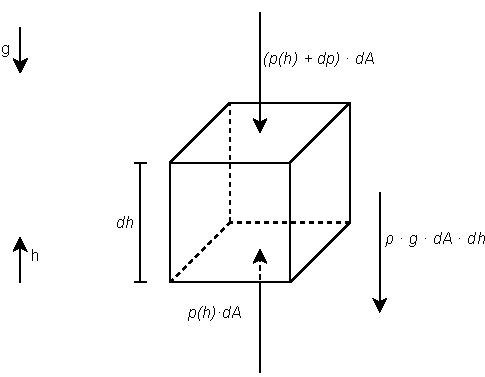
\includegraphics[width=.4\textwidth]{baro_dgl.drawio}
    \caption{Forces around a finitesimally small element}
    \label{fig:baro_FE}
\end{figure}



quick derivation of barometric formula based on the pressure pde.


Resulting from the equilibrium around a finitesimally small element in figure \ref{fig:baro_FE}.


follows the force equilibrium for force terms as well as the gravity term

\begin{equation}
    \sum{F_h} = 0 = p(h) \cdot dA - ( p(h) + dp )\cdot dA -  \rho \cdot g \cdot  dh \cdot dA
    \label{eq:baro_equilibrium}
\end{equation}

resolves into:
\begin{equation}
    dp=-\rho \cdot g\cdot dh
    \label{eq:baro_equilibrium_simple}
\end{equation}

with ideal gas formula

\begin{equation}
    \frac{dp}{p} = \frac{-g}{R \cdot T} \cdot dh
    \label{eq:baro_equilibrium_perfect}
\end{equation}

and T = f(h) from Interational Standard Atmosphere ISA-correlation
\begin{equation}
    T(h)= a  \cdot h + T_0
    \label{eq:isa_temperature}
\end{equation}

with a being defined as dT/dh and -6.5 K/km for the troposphere. See Table \ref{tab:isa_temp}
Since Temperature behaviour is defined by the \textcite{iso_standard_1975}  within the ISA as follows:
\
perhaps mention troposphere, strato, pause,... here

\begin{table}[h]
    \centering
    \begin{tabular}{@{}lccc@{}}
        \toprule
        Atmospheric Layer & Geopotential Altitude {[}km{]} & Temperature T at bottom {[}K{]} & Temperature gradient a {[}K/km{]} \\ \midrule
        Troposphere       & -2-0                           & 301.15                          & -6.5                              \\
        Troposphere       & 0-11                           & 288.15                          & -6.5                              \\
        Tropopause        & 11-20                          & 216.65                          & 0                                 \\
        Stratosphere      & 20-32                          & 216.65                          & 1                                 \\
        Stratosphere      & 32-47                          & 228.65                          & 2.8                               \\
        Stratopause       & 47-51                          & 270.65                          & 0                                 \\
        Mesosphere        & 51-71                          & 270.65                          & -2.8                              \\
        Mesosphere        & 71-80                          & 214.65                          & -2                                \\ \bottomrule
    \end{tabular}
    \caption{International Standard Atmosphere cite ISO75}
    \label{tab:isa_temp}
\end{table}


\begin{equation}
    \frac{dp}{p}=\frac{-g}{R*(a*h+T_0)}*dh
    \label{eq:baro_pde_full}
\end{equation}
\begin{equation}
    \ln(\frac{p}{p_0}) = - \frac{g}{a \cdot R} \cdot ln(\frac{a*h+T_0}{a*h_0+T_0})
    \label{eq:baro_integrated}
\end{equation}
\begin{conditions}
    a & $p/p_0$                                                                                                \\
    b & $\frac{-g}{a \cdot R} $                                                                                \\
    c & $\frac{a*h+T_0}{a*h_0+T_0} = 1+ \frac{a \cdot (h-h_0)}{a*h_0+T_0} = 1+ \frac{a \cdot (h-h_0)}{T(h_0)}$
    \label{eq:baro_substitutions}
\end{conditions}

\begin{equation}
\ln(a) = b * \ln(c) = \ln(c^b)
\label{eq:baro_sub_first}
\end{equation}
\begin{equation}
\rightarrow a = c^b$$
\label{eq:baro_sub_last}
\end{equation}
\begin{equation}
    \frac{p}{p_0}=\left(1+\frac{a \cdot\left(h-h_0\right)}{T\left(h_0\right)}\right)^{\frac{-g}{a \cdot R}}
    \label{eq:baro_Tvar}
\end{equation}

\begin{conditions}
    p      & pressure at current altitude [Pa]                                \\
    p_{0}  & reference pressure [Pa]                                          \\
    h      & current altitude   [m]                                              \\
    h_{0}  & reference altitude [m]                                           \\
    T(h_0) & temperature at reference altitude[K]                             \\
    a      & ISA Temperature Coefficient depending on altitude (-6.5e-3)[K/m] \\
    g      & gravity constant (9.80665) [m/s^2]                               \\
    R      & Ideal Gas Constant  (287.05287)[m^2/( K\cdot s^2)]
\end{conditions}

This formula however is not valid for $a=0$. So the barometric pde \ref{eq:baro_pde_full} needs to adapted before integration. From equation \ref{eq:baro_pde_full} follows equation \ref{eq:baro_Tconst_pde}. Integrating then yields \ref{eq:baro_Tconst_integrated} which results into \ref{eq:baro_Tconst}, the barometric equation for a constant temperature coefficient.
\begin{equation}
    $$dp/p = -g/(R*T_0)*dh$$
    \label{eq:baro_Tconst_pde}]
\end{equation}
\begin{equation}
    $$ln(p/p_0) = -g/(R*T_0)*h$$
    \label{eq:baro_Tconst_integrated}
\end{equation}
\begin{equation}
    \frac{p}{p_0}= exp\left(\frac{-g}{RT(h_0)}\cdot(h-h_o)\right)
    \label{eq:baro_Tconst}
\end{equation}

Since the desire to acquire the altitude h from pressure has not receeded, the next step is transforming the barometric equation for $a\neq0$ \ref{eq:baro_Tvar} into a function of the altitude.

resolving into a function of h
$$ln(\frac{p}{p_0}) =\frac{-g}{RT(h_0)}\cdot(h-h_o) $$

\begin{equation}
    h = ln(\frac{p}{p_0})\cdot \frac{RT(h_0)}{-g}+h_0
    \label{eq:h_baro_Tconst}
\end{equation}


Now, using equation \ref{eq:baro_Tvar} for $a\neq0$ to calculate altitude as a function of pressure:

\[
    1 + \frac{a}{T(h_0)}\cdot (h-h_0) = \left(\frac{p}{p_0}\right)^{\frac{1}{\frac{-g}{a \cdot R}}}
\]

\begin{equation}
    \rightarrow h = \left(\frac{p}{p_0}^{\frac{-a*R}{g}}-1\right)\frac{T(h_0)}{a}+h_0
    \label{eq:h_baro_Tvar}
\end{equation}
Formula \ref{eq:h_baro_Tvar} is the equation used for ISA-assumptions within a atmospheric layer with temperature change.

in aerospace context this gets used as follows.

$p_0$ is the reference pressure which gets used in conjunction with $T_0$.

Based upon reference pressure, the pressure value in at the boundary levels can be estimated.


If altitude gets calculated, it needs to follow in two steps.
Based on ideal temperature at sea level

1. determine which ISA-Level is present by determining p/p_0 at the boundaries.
$p/p_0 = f(h)$)


2. base calculation off of isa reference level
p/p

$$(a*h/T_0+1)/(a*h_0/T(h_0+1)$$


TODO: implement g as a function of lat and long


For further use, the barometric formula will be expressed as  $$h = f(p,p_0)$$

in accordance to ISO75 the altitude is the geopotential altitude which is equivalent to the orthometric height and MSL.

Also available is the geometric altitude which references the earth ellipsoid as its base and which is generally used by geodetic applications as a geometrically reliable reference system.


\section{Finding a reference state}
Goal of this work is finding a reference frame for all parameters into which they can be transformed into and back.

A starting point which shall be considered is the geodetic reference.

it measures the aircraft's position by its displacement from the previously (ref?) discussed WGS84 system.

Meaning that altitude gets measured as the orthometric height (see ellipsoid height-geoid height).

Latitude and Longitude form the x and y axis of the COS. True heading forms the reference heading within the geodetic system.

All aircraft parameters related to motion and position of the aircraft should be attempted to be condensed into this form.


\section{error detection and mitigation}

Examination of Receiver autonomous integrity monitoring (RAIM) from GNSS applications.


basic principle
1 in 1 out
basic


2 in 1 out
mean solution. Detect discrepancies
1. simple solution: take average
2. detect discrepancies but still take average

3+ in 1 out.
1. take average
2. detect value with strong variations and isolate (it is assumed that only 1 sensor is faulty)
2.1 predict value and deny value if it is larger than 3 times standard deviation (Wen07, 239).

implementation details. see [Bro92]


\chapter{Implementation}


\section{Software architecture considerations}

Careful consideration needs to be given to the workflow of the level 1 check to allow scalability and minimal manual interaction in later stages. To achieve this architecture, manual steps are reduced as far as possible. However, some level of configuration must be implemented. Otherwise only relational sensor behaviour could be detected. Meaning that sensor faults occuring temporarily within an experiment can be detected but permanent behaviour is not noticed by a relative algorithm


\section{Level 1 Implementation}

For implementing the level 1 checks, the measured data needs to be compared to the expected data. To gain insight into what the the expected data is, the configuration file of the data acquisitioning system needs to get parsed.
Luckily, the DAQ's format is a .zip directory.
The 7zip command line tool gets used for opening the configuration file since the configuration file's format is not fully complying to the zip standard making several python libraries fail during the process. This stems from an issue with the zip header and footer parts of the file that are not at expected places (i.e.\ the front the back).
Once opened, the configuration file contains multiple files as well as an essential xml file that contains the needed sensor metadata.

Missing datasets can now easily be found by comparing the expected values from the configuration file to the actual generated data.

For the second step.


\section{Level 2 Implementation}

Since the IMC DAQ System resamples the 20Hz Sensors to a straight timeframe data gets lost in the process. This makes potentially noisy sensors output the same value twice in a row since the DAQ hasn't yet received the new sensor data and outputs the same value multiple times in a row. Even sensors with a high noise ratio such as the fine part of a gps latitude signal outputs the same value twice in a row which is highly unlikely to happen on a statistical basis. Since this occurs quite often the question arises if the actual sampling may be lower than the actual data.


\section{Level 3 Implementation}

Aims of Level 3 Implementation are to model the aircraft's state in a reference system.
This reference system shall be geodetic and fixed to the earth while the aircraft moves through it. Moving aircraft coordinate systems like the aerodynamic and the along track Coordinate system may be derived from its geodetic position using ?angles and velocities.


Interfacing: Clean interfaces are generated throughout the model. Enabling a standardized state vector x. Meaning that A remains standardized for any aircraft while B, U and L need to be adjusted for any changes to the aircraft or sensor data.

The integration step may be omitted in early design stages since the necessary equations and equilibriums of Forces and Moments could only be modelled linearly while neglecting various unknown factors like shifting CG due to fuel burn, actual Inertia of Aircraft and aicraft mass. Hence, this step may be implemented if time allows it.


\section{Examining Altitude Sensors}

As seen in~\ref{fig:gps_diff} gps altitudes have a base mean value of difference of about 3-4 meters. During flight level changes the base level changes significantly. Further investigation is needed how these changes may arise.

One possible approach would be considering different placements of gps antennas within the airframe. since the IMAR's position is precisely known and lies around the center of gravity but the ASCB's gps position is not known exactly the process is not facilitated. However using the process of lever arms the position could be roughly estimated and compensated from the altitude difference in figure \ref{fig:gps_diff}.

\begin{figure}[h]
    \centering
    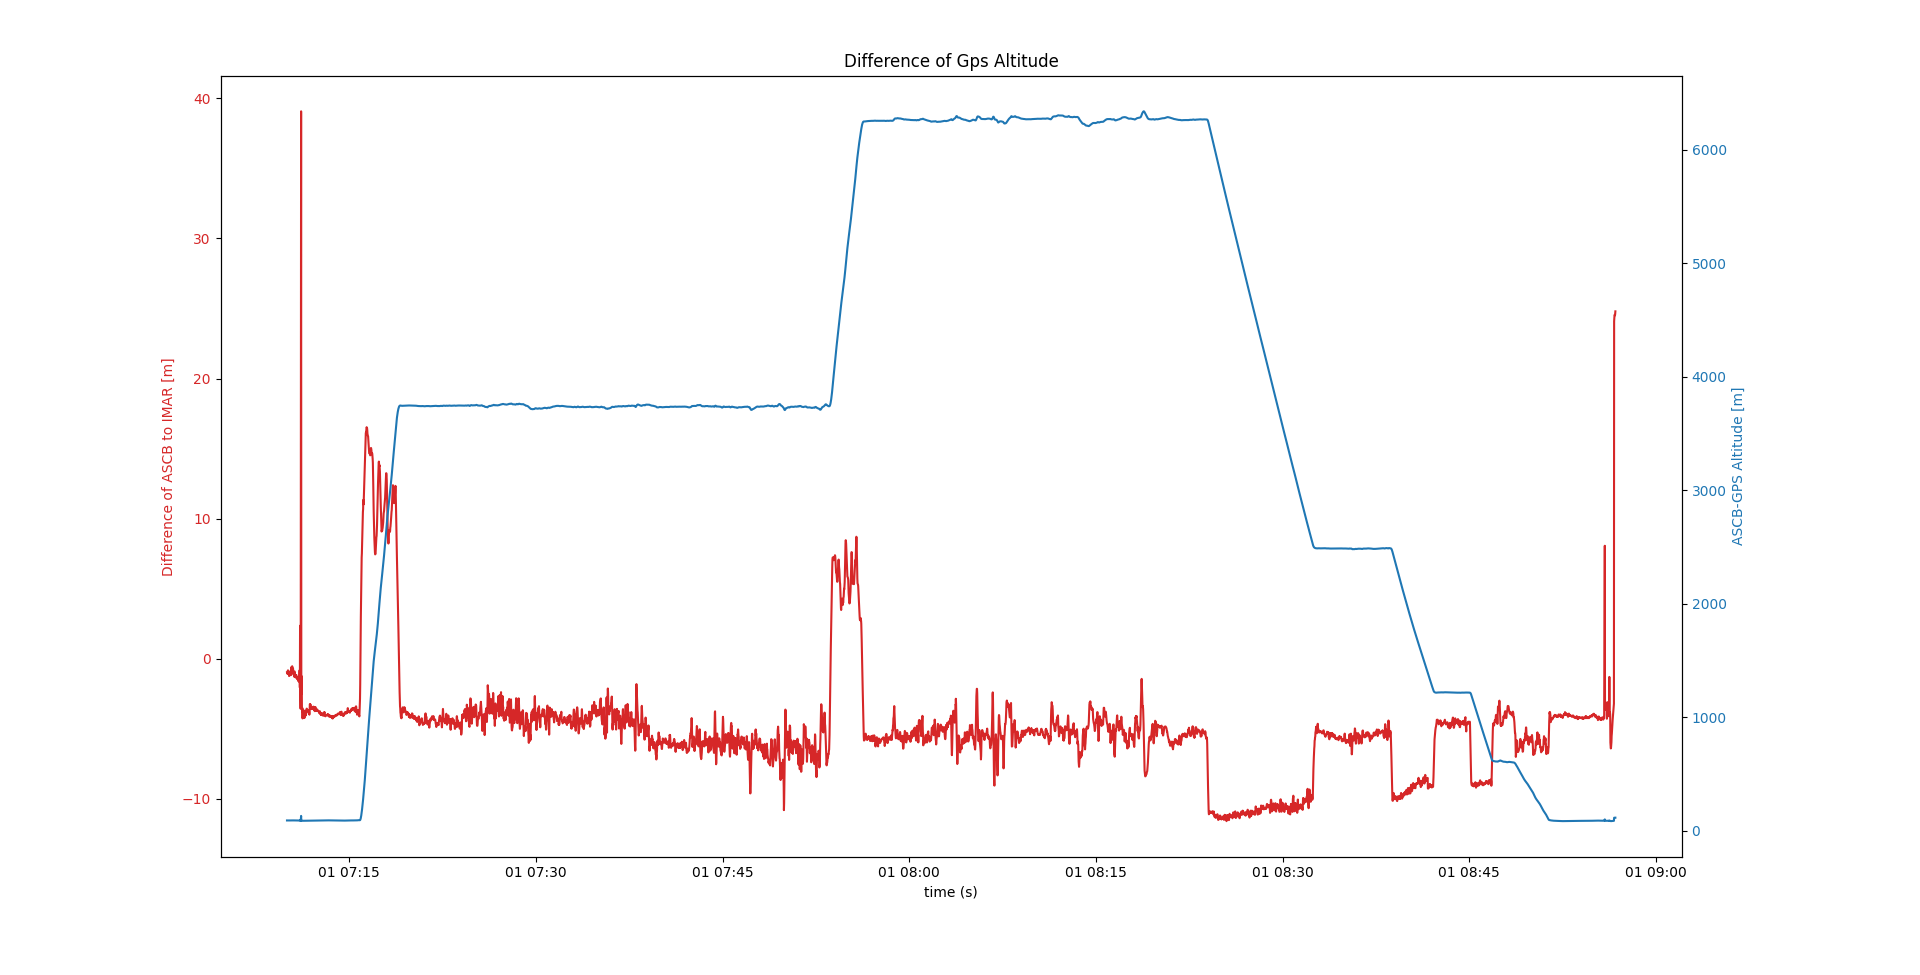
\includegraphics[width=.8\textwidth]{gps_difference_imar_ascb}
    \caption{GPS difference for the aircraft base platform (ASCB) as well as experimental sensor (IMAR)}
    \label{fig:gps_diff}
\end{figure}

Another incurring deviation is investigating the ~40m/150ft offset for gps altitudes. Possible causes may be Uncorrected Ellipsoid gnss altitudes. However, this appears unlikely since generally the offset in the region would be added and not subtracted [further investigation needed].


Difficulty diagnosing sensors without previous knowledge. limitations within sensor behaviour. Checks include: range, too much sensor movement, too few sensor movement.

Relative examinations possible for errors occuring for finite time within experiment but not if all of the experiment data is corrupt.





